The Sybil attack is coined by Douceur\cite{douceur2002sybil} in 2002 in the
context of peer-to-peer systems. In this section, we introduce the key
theoretical results and the definitions used in the remainder of this survey.

\subsection{Theoretical Results}\label{sec:sybil-theory}
Douceur defined the Sybil attack as forging multiple identities under the same
entity\cite{douceur2002sybil}. An entity can be for example a physical user of
the system and identities are how entities present themselves to the system.
Thus a local entity has no direct knowledge of remote entities, only their
identities. The forged identities do not necessarily follow the protocol
specified by the underlying network, i.e. they assume the characteristics of
Byzantine fault\cite{lamport1982byzantine}.
% We use these terms in the remainder of the survey.

The author modelled the system as a general distributed computing environment
where there is no constraint on the topology, every node has limited
computational resources and messages are guaranteed to be delivered. Under this
model, the author proved that the Sybil attack is always possible without a
central, trusted authority.

% Preventing the Sybil attack is in fact a lot
% more difficult because peer-to-peer systems often do not have a central, trusted
% authority.

Cheng and Friedman proved a similar result in the context of reputation
systems\cite{cheng2005sybilproof}. Reputation systems are commonly used in
e-commerce websites and the internet in general, where identities are rewarded
by their good behaviour or usefulness. Google's PageRank\cite{page1999pagerank}
is an example of a reputation system, where a large number of links to a website
makes it more reputable. It was formally proven that peer-to-peer reputation
systems cannot be made to prevent the Sybil attack, it is only possible prevent
it by using trusted parties.

% Cheng and Friedman proved an important result regarding the Sybil attack in
% reputation systems\cite{cheng2005sybilproof}. Reputation systems are commonly
% used in MANET, e-commerce and the internet in general, where entities are
% rewarded by their good behaviour and penalised otherwise. Google's
% PageRank\cite{page1999pagerank} is an example of a reputation system, where a
% large number of links to a website makes it more reputable. Cheng and Friedman
% classified reputation systems into two categories,
% \begin{enumerate}
% \item symmetric reputation systems where the reputation score only depends on
%   the network topology, popular reputation mechanisms such as
%   PageRank\cite{page1999pagerank} and EigenTrust\cite{kamvar2003eigentrust} are
%   examples of symmetric reputation systems, and
%     \item asymmetric reputation systems where there some nodes are trusted and
%       reputation scores are propagated through the trusted nodes, most OSN are
%       examples of asymmetric reputation systems.
% \end{enumerate}
% The authors formally proved that symmetric reputation systems are vulnerable to
% the Sybil attack. But in the asymmetric case, it is possible to construct a
% Sybil-proof reputation system.

\subsection{Model and Definitions}
One of the common models, especially in the context of online social networks,
is shown in \autoref{fig:attack-edge}. It is first introduced by the authors of
SybilGuard\cite{yu2006sybilguard}. Nodes inside the left region are identities
created by honest entities, the edges connecting those nodes are real-world
trust relationships. The right region contains the Sybils and they are connected
with fake relationships. The edges connecting the two regions are called
\emph{attack edges}. These can be created by tricking an honest user to befriend
a Sybil, stealing an honest user's account and so on. Many Sybil defence
mechanisms rely on the fact that attack edges are difficult to create as we will
describe in \autoref{sec:defences}.

\begin{figure}
  \centering
  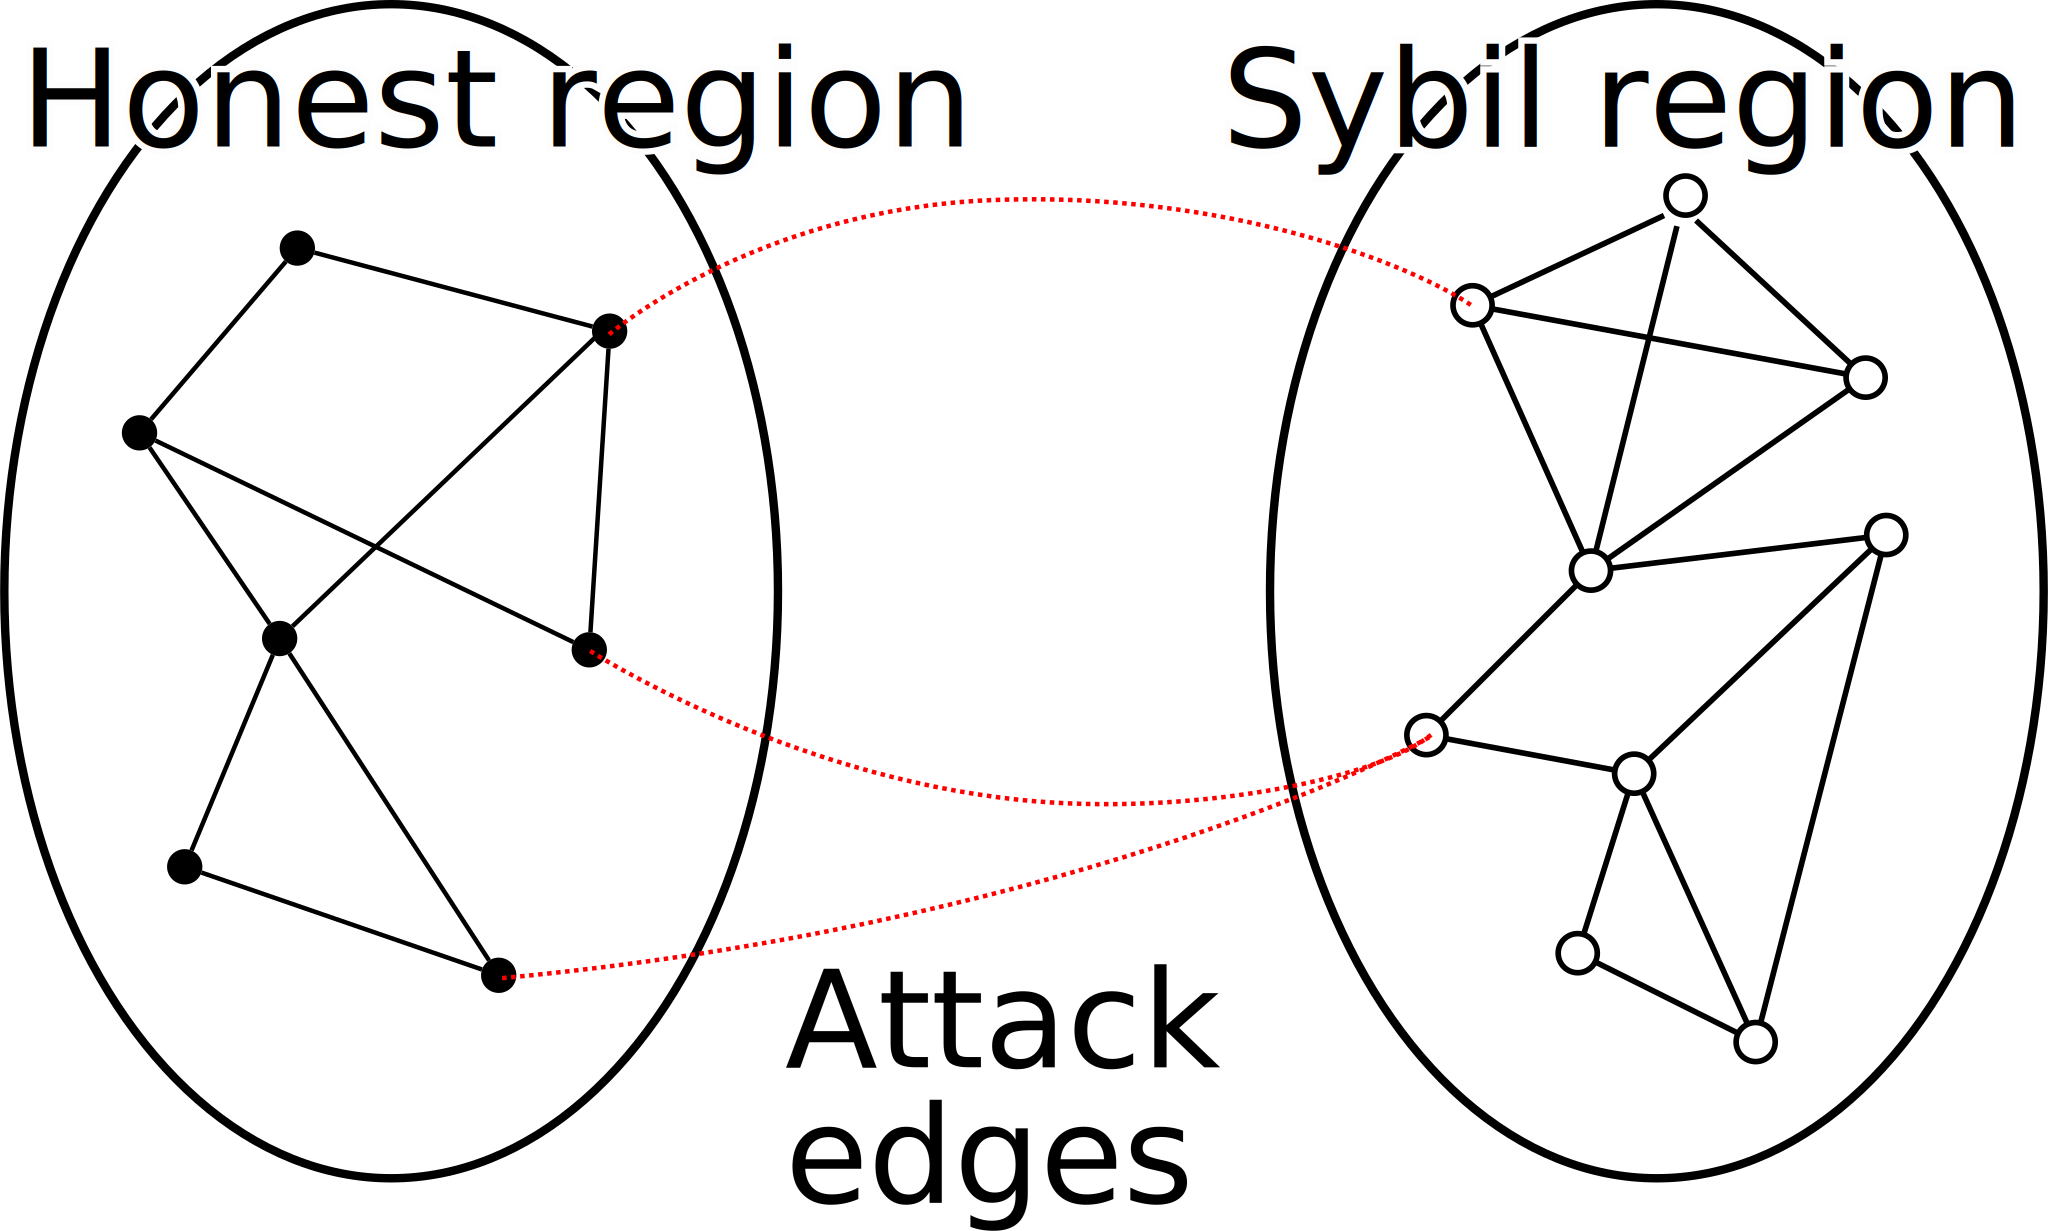
\includegraphics[width=0.4\textwidth]{attack_edges}
  \caption{Visualisation of the Sybil attack in online social networks}
  \label{fig:attack-edge}
\end{figure}


%%% Local Variables:
%%% mode: latex
%%% TeX-master: "main"
%%% End:
